\subsection{Vergleich zum O(1)-Scheduler}\label{s:compO1}
Anmerkung: noch leer, da noch keine geeignete Literatur gefunden
 \cite{asilberschatz}  Seite 211 following, kurze erklärung zum O(1)
 
  CFS uses the fair clock and wait runtime to keep all the runnable tasks sorted by the rq->fair\_clock - p->wait\_runtime key in the rbtree (see the Red-Black Tree sidebar). So, the leftmost task in the tree is the one with the “gravest CPU need”, and CFS picks the leftmost task and sticks to it. As the system progresses forward, newly awakened tasks are put into the tree farther and farther to the right—slowly but surely giving every task a chance to become the leftmost task and, thus, get on the CPU within a deterministic amount of time.
 
 Because of this simple design, CFS no longer uses active and expired arrays and dispensed with sophisticated heuristics to mark tasks as interactive versus non-interactive.
 
 CFS implements priorities by using weighted tasks—each task is assigned a weight based on its static priority. So, while running, the task with lower weight (lower-priority) will see time elapse at a faster rate than that of a higher-priority task. This means its wait\_runtime will exhaust more quickly than that of a higher-priority task, so lower-priority tasks will get less CPU time compared to higher-priority tasks. 
 \cite{cpabla}
 
 
 Paper 2008 International Symposium on Information Technology
 \cite{papercomparison}
 
\begin{figure}[h]
	\centering
	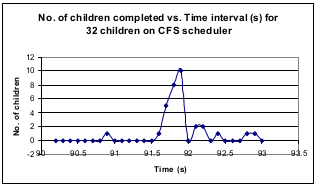
\includegraphics[width=0.45\textwidth]{pictures/fairness_32_cfs.png}
	\caption{Fairness-Messung für 32 Kinprozesse im CFS Scheduler.}
	\label{fig:fair_meas_cfs}
\end{figure}
\begin{figure}[h]
 	\centering
 	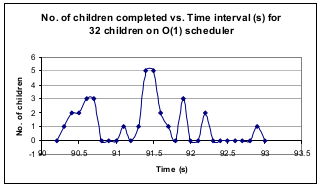
\includegraphics[width=0.45\textwidth]{pictures/fairness_32_O1.png}
 	\caption{Fairness-Messung für 32 Kinprozesse im O(1) Scheduler.}
 	\label{fig:fair_meas_o1}
\end{figure}
 
\begin{figure}[h]
 	\centering
 	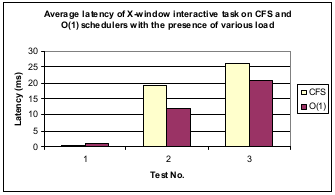
\includegraphics[width=0.45\textwidth]{pictures/avg_latency.png}
 	\caption{Durchschnittslatenz in CFS und O(1) Scheduler.}
 	\label{fig:avg_latency}
\end{figure}

\begin{figure}[h]
 	\centering
 	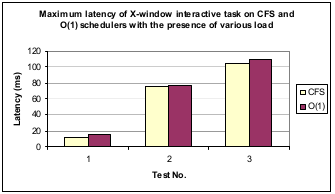
\includegraphics[width=0.45\textwidth]{pictures/max_latency.png}
 	\caption{Durchschnittslatenz in CFS und O(1) Scheduler.}
 	\label{fig:max_latency}
\end{figure}